% SPDX-FileCopyrightText: 2026 Cyprien PIERRE
% SPDX-License-Identifier: CC-BY-4.0
\documentclass[tikz,border=5pt]{standalone}
\usepackage[T1]{fontenc}
\usepackage{lmodern}
\usetikzlibrary{arrows.meta,positioning}
\begin{document}
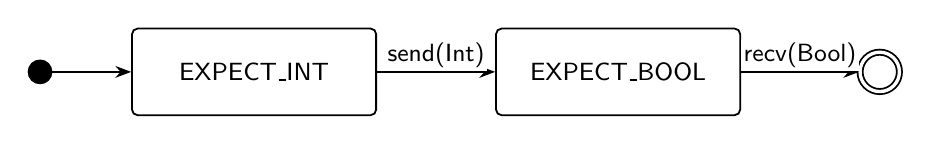
\begin{tikzpicture}[
  font=\sffamily\small,
  initial/.style={circle, fill=black, draw=black, minimum size=3mm, inner sep=0pt},
  state/.style={draw, rounded corners=2pt, minimum height=11mm, minimum width=31mm,
    align=center, line width=.65pt},
  final/.style={circle, draw, double, double distance=1.2pt, minimum size=5mm,
    inner sep=0pt, line width=.65pt},
  transition/.style={-{Stealth[length=2mm]}, line width=.7pt}
]
\node[initial] (start) {};
\node[state, right=10mm of start] (int) {EXPECT\_INT};
\node[state, right=15mm of int] (bool) {EXPECT\_BOOL};
\node[final, right=15mm of bool] (done) {};
\draw[transition] (start) -- (int);
\draw[transition] (int) -- node[above, fill=white, inner sep=1pt] {send(Int)} (bool);
\draw[transition] (bool) -- node[above, fill=white, inner sep=1pt] {recv(Bool)} (done);
\end{tikzpicture}
\end{document}